\documentclass[review,11pt]{elsarticle}
%\documentclass[preprint,review,12pt,authoryear]{elsarticle}
\usepackage{lineno,hyperref,ulem,todonotes}
\usepackage{rotating}
\usepackage{amsmath}
\modulolinenumbers[5]
%\usepackage{natbib}
\journal{Computational Geosciences}

%%%%%%%%%%%%%%%%%%%%%%%
%% Elsevier bibliography styles
%%%%%%%%%%%%%%%%%%%%%%%
%% To change the style, put a % in front of the second line of the current style and
%% remove the % from the second line of the style you would like to use.
%%%%%%%%%%%%%%%%%%%%%%%

%% Numbered
\bibliographystyle{model1-num-names}

%% Numbered without titles
%\bibliographystyle{model1a-num-names}

%% Harvard
%\bibliographystyle{model2-names.bst}\biboptions{authoryear}

%% Vancouver numbered
%\usepackage{numcompress}\bibliographystyle{model3-num-names}

%% Vancouver name/year
%\usepackage{numcompress}\bibliographystyle{model4-names}\biboptions{authoryear}

%% APA style
%\bibliographystyle{model5-names}\biboptions{authoryear}

%% AMA style
%\usepackage{numcompress}\bibliographystyle{model6-num-names}

%% `Elsevier LaTeX' style
%\bibliographystyle{elsarticle-num}
%%%%%%%%%%%%%%%%%%%%%%%

\begin{document}

\begin{frontmatter}

\title{Subgrid Model for Microtopography Effect on Surface Flow}

%\author[ornl]{Ahmad Jan \corref{cor}} \author[lanl1]{Ethan T. Coon} \author[ornl]{Scott L. Painter} \author[lanl2]{Rao Garimella} \author[lanl2]{J. David Moulton}

%\address[ornl]{Climate Change Science Institute and Environmental Sciences Division, Oak Ridge National Laboratory, Oak Ridge, Tennessee, USA\fnref{copyrightnotice}} 
%\address[lanl1]{Computational Earth Sciences Group, Earth and Environmental Sciences Division, Los Alamos National Laboratory, Los Alamos, New Mexico, USA} 
%\address[lanl2]{Applied Mathematics and Plasma Physics Group, Theoretical Division, Los Alamos National Laboratory, Los Alamos, New Mexico, USA} 


%\cortext[cor]{Corresponding Author: Ahmad Jan; Email: jana@ornl.gov; Phone: (865) 576-8175.}



\begin{abstract}
This article presents a subgrid model to represent accurate surface flow behavior, influenced by surface microtopography, at large spatial scales. The spatial heterogeneity in the surface microtopography plays an important role in the surface water retention, the runoff, and surface/subsurface interactions, and thereby significantly affects the shape of the hydrographs. For watershed-scale simulations, the accumulation term and the flow law in the governing equation of the surface flow need to be altered to incorporate the effect of surface microtopography on the water storage and the discharge rate. Our subgrid model incorporates high-resolution spatial configuration of the surface topography to capture the fine-scale behavior of the surface runoff at the watershed-scale(??). Numerical results of the subgrid model are compared with the no subgrid model and the fine-scale simulations of five ice-wedge polygons. A good match between the fine-scale simulations and the subgrid model results confirms that our subgrid model improved the shape of the hydrographs and the total water content in the system. Furthermore, the model is applied to a 468 polygons catchment, and significant changes are observed in the results of with and without subgrid model. The results of the developed model highlight that the model is able to achieve fine-scale behavior at larger spatial scales.
\end{abstract}

\begin{keyword}
%Mixed-dimensional model\sep Permafrost thermal hydrology  \sep Integrated surface/subsurface flow modeling \sep Arctic 
Subgrid model \sep Permafrost \sep Hydrology  \sep Hydrograph \sep Watershed
\end{keyword}


\end{frontmatter}

\linenumbers

\section{Introduction}\label{introduction}
To gain insight into the role of heterogeneous spatial structure of the ground surface is important for understanding interactions between surface and subsurface, surface runoff and discharge rate. Numerical models must be able to incorporate fine-scale spatial variability through a subgrid model representation when conducting simulations with low resolution grids -- an extended version of the existing models is required to account for fine-scale surface flow behavior. 

When rainfall dominates the infiltration, surface runoff happens. The surface runoff and the shape of the hydrographs could significantly be affected by the spatially varying surface microtopography (unevenness at small scale). The importance of the microtopograhy  cannot be ignored for accurate representation of the surface processes. From simulations perspective, an accurate flow behavior is captured at the fine-scale (a scale of centimeters), however, fine-scale simulations are computationally expensive. In addition, most of the field observations are made at the fine-scale, and the lack of high spatial resolution data at the watershed scale, surface microtopograhic effects on the runoff are usually ignored at larger spatial scales. A subgrid model is build on the information gained from highly resolved surface topographic data; the depressions and obstructions. Depressions are disconnected low points in the topography (surface pits) and retains water that is available only for infiltration or/and evaporation. On the other hand, obstructions exits above the depressions and interrupt and slow the flow, but do not completely block it. To capture these effects in a model, the depressions require to change the accumulation term and obstructions need to introduce a friction factor to influence the surface flow term and hence surface detention.

The integrated suface/subsurface modeling has received considerable attention from researchers across the world; see, for example,~\cite{painter2013modeling,kurylyk2014climate,spainter2016integrated} and references therein. Here we focus only on the subgrid modeling approach. 
The significance of the surface microtopographic features are well described in~\cite{stammers1956effect}. Panday and Huyakorn (\citeyear{panday2004fully}) presented an integrated surface/subsurface flow model with subgrid representation through the surface depressions and obstructions.

The rest of the paper is organized as follows. Section~\ref{subgridmodel} introduces the derivation of the governing equations of the subgrid model. A short description, for a quick reference, of the Advanced Terrestrial Simulator (ATS) and the Arcos multiphysics management framework, within which we implemented our subgrid model, is presented in Section~\ref{ATS}. In Section~\ref{numerical-tests} we compare the numerical results of our subgrid model with no subgrid model and fine-scale results to illustrate the accuracy of our subgrid model for capturing fine-scale microtopographic features. Finally, in Section~\ref{conclusion}, we offer closing remarks and future research inline with thaw-induced subsidence.

%Section~\ref{motivation} presents some fine-scale simulation results and analysis that motivated the approach.  In Section~\ref{mixed-dim-model} we introduce our mixed-dimensional modeling approach, loosely coupled scheme and the ATS refactoring strategy.

%The surface flow is mainly affected by the depressions and obstructions -- characteristic of the microtopograpy. 

%Insight into spatial patterns of groundwater discharge through evapotranspiration is critical for understanding responses of groundwater dependent ecosystems


\section{Subgrid Model}\label{subgridmodel}
This section describes the derivation of the subgrid model. The subgrid model alters the accumulation term and the flow law. For example, the ponded depth in the accumulation term is typically replaced with a volumetric depth, the ponded depth that would occur if the surface were flat. Specifically, we make the substitution in the accumulation term, where is ponded depth. The volumetric head may be calculated on geometric arguments. Specifically, if the microtopographic elevation field on an ice-wedge polygon (IWP) is $Z_*(x,y)$, the the volumetric depth is
\begin{equation}\label{volumetric-depth1}
\Phi (\delta) = \frac{1}{A} \iint \left( \delta + Z_0 - Z_*(x,y) \right ) H \left( \delta + Z_0 - Z_*(x,y) \right ) dx dy
\end{equation}
Where the integration is over the surface of the IWP, $A$ is the area of the IWP, $Z_0$ is the minimum elevation in the IWP, and $H$ is the Heaviside function. This could be computed from the microtopography and stored as a lookup table. Or, we could employ a simpler parameterization. To that end, we consider parameterizing the microtopography with two parameters: (1) the elevation range spanned by the subgrid microtopography $\delta_\text{max}$, and (2) the specific excluded volume $\delta_\text{ex}$, which is the soil volume per unit bulk area. Then, we approximate the volumetric depth as

\begin{equation}\label{volumetric-depth2}
\Phi (\delta) =
\begin{cases} (2 \delta_\text{max} - 3 \delta_\text{ex}) \left(\frac{\delta}{\delta_\text{max}} \right )^2 + (2 \delta_\text{ex} -  \delta_\text{max}) \left(\frac{\delta}{\delta_\text{max}} \right )^3 & \text{if} \hskip 0.1in 0 \leq \delta \leq \delta_\text{max}, \\
\delta - \delta_\text{ex} & \text{if} \hskip .1in \delta > \delta_\text{max}.
\end{cases}
\end{equation}
The IWP shown in Fig~\ref{3Dpolygon40} was used to evaluate the parameterization Equation~\ref{volumetric-depth2}. The volumetric depth calculated from the approximation Equation~\ref{volumetric-depth2} is compared (curve) with the direct calculation Equation~\ref{volumetric-depth1} (dots) for an ice-wedge polygon in Figure~\ref{polygons}. Also, shown is the volumetric depth in the absence of microtopography, which is linear with slope unity. Equation~\ref{volumetric-depth1} is a very good approximation.
Microtopographic effects on the flow law are not as straightforward to incorporate as the volumetric head $\Phi(\delta)$. In particular, we should make the distinction between depressions and obstractions (Panday and Huyakorn, 2004). Depressions are disconnected low points in the topography. The ponded depth must rise above the level of those depressions before any flow can happen. Obstructions exist above the depressions and interrupt and slow the flow, but do not block it completely.
To model the effects of obstructions and depressions, we propose the following modification to the flow law
\begin{equation}
U = - \Theta(\delta) \frac{(\delta - \delta_\text{d})^{2/3}}{n_\text{mann} (\| \nabla Z \| +\epsilon)^{1/2}}
\end{equation}
where $\delta_\text{d}$ is the depression depth, and $\Theta(\delta) \in [0,1]$ is a fractional conductance which account for flow reduction by obstructions.

\begin{figure}
\centering
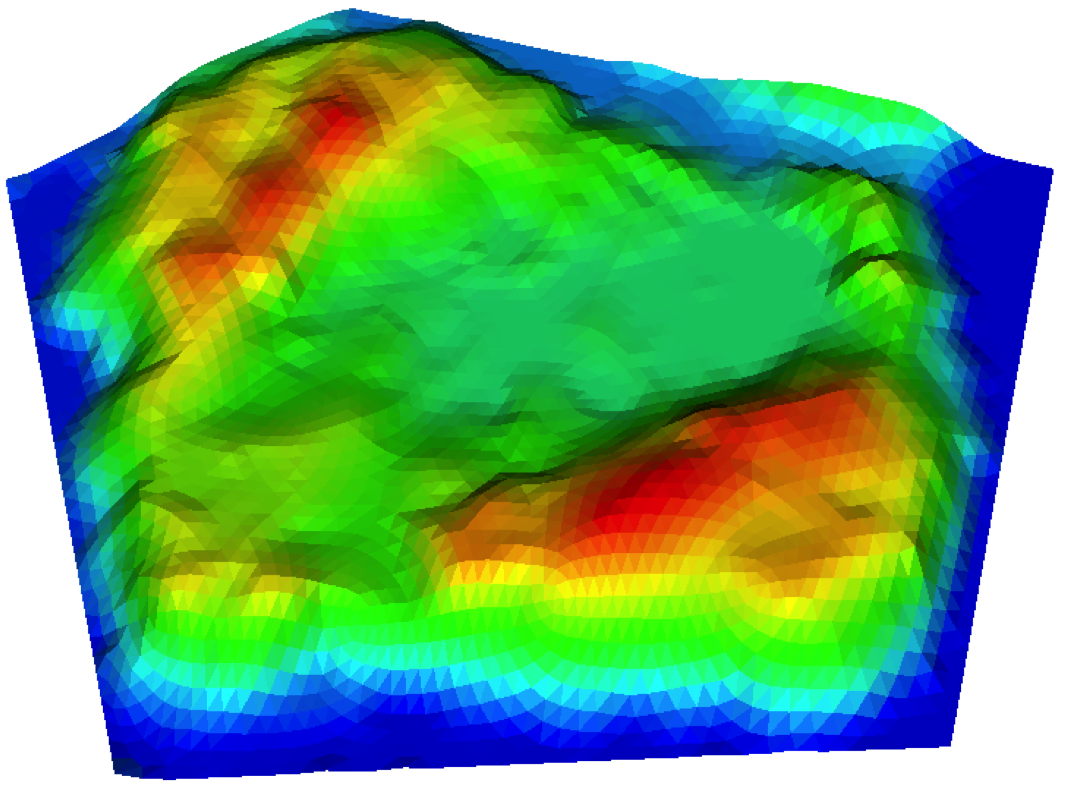
\includegraphics[width=11cm, height=6cm]{3DPolygonsImages/3Dpolygon40.png}
\caption{Microtopograpy for an example ice-wedge polygon from the Barrow Environmental Observatory (BEO).}
\label{3Dpolygon40}
\end{figure}

\begin{figure}
\centering
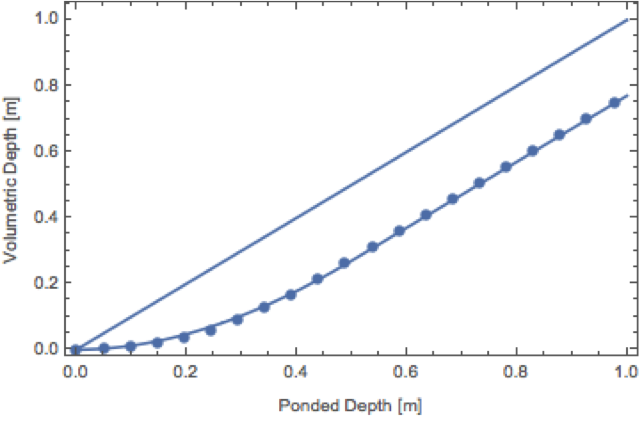
\includegraphics[width=12cm, height=8cm]{3DPolygonsImages/polygon40.png}
\caption{Volumetric depth versus ponded depth for polygon shown in Figure~\ref{3Dpolygon40}.}
\label{polygon40}
\end{figure}

\begin{figure}
\centering
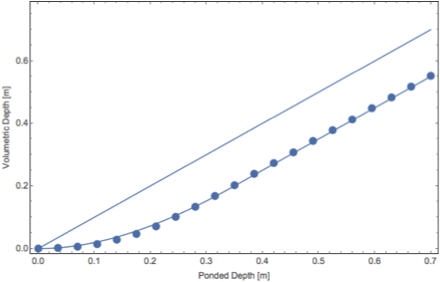
\includegraphics[width=6cm, height=6cm]{3DPolygonsImages/picture2.png}
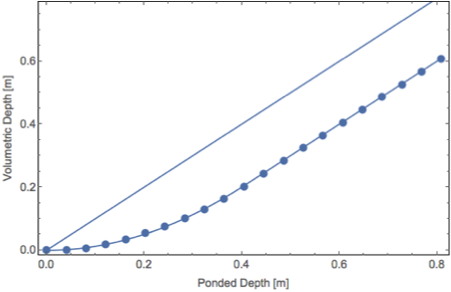
\includegraphics[width=6cm, height=6cm]{3DPolygonsImages/picture3.png}\\
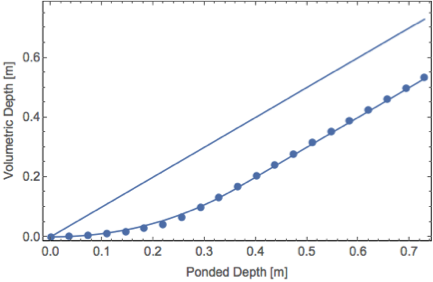
\includegraphics[width=6cm, height=6cm]{3DPolygonsImages/picture4.png}
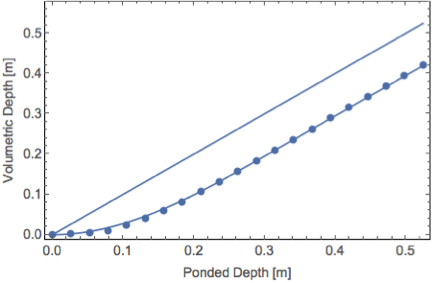
\includegraphics[width=6cm, height=6cm]{3DPolygonsImages/picture5.png}
\caption{Volumetric depth versus ponded depth for four additional ice-wedge polygons.}
\label{polygons}
\end{figure}

To calculate $\delta_\text{d}$ from the microtopography, we now propose an approach based on site percolation. Specifically, we fill the lowest elevation surface cells until the cluster of inundated cells spans the IWP. This is the percolation threshold. The water height at the percolation threshold defines the $\delta_\text{d}$. Figure~\ref{perc-cluster-poly40} shows the spanning cluster at the percolation threshold for the IWP of Figure~\ref{3Dpolygon40}. The depression depth calculated this way is 4.1 cm for this IWP.
It is reasonable to assume that the fractional conductance is well approximated by the fractional cross section available to flow, which can be estimated as the ratio of volumetric depth to ponded depth.

\begin{equation}
\Theta {(\delta_\text{d})} \approx \frac{( \Phi (\delta) - \Phi (\delta_\text{d}))} {\delta} H \left( \delta - \delta_\text{d}\right )
\end{equation}
Where $H$ is the Heaviside function. The numerator is the flowing cross sectional area. Note the velocity is multiplied by ponded depth to get a flux, so the molar flux appearing in the conservation equations becomes

\begin{equation}
\eta_{l} \delta U = - \eta_l  ( \Phi (\delta) - \Phi (\delta_\text{d})) H \left( \delta - \delta_\text{d}\right ) \Theta(\delta) \frac{(\delta - \delta_\text{d})^{2/3}}{n_\text{mann} (\| \nabla Z \| +\epsilon)^{1/2}} \nabla(Z + \delta)
\end{equation}
\begin{figure}
\centering
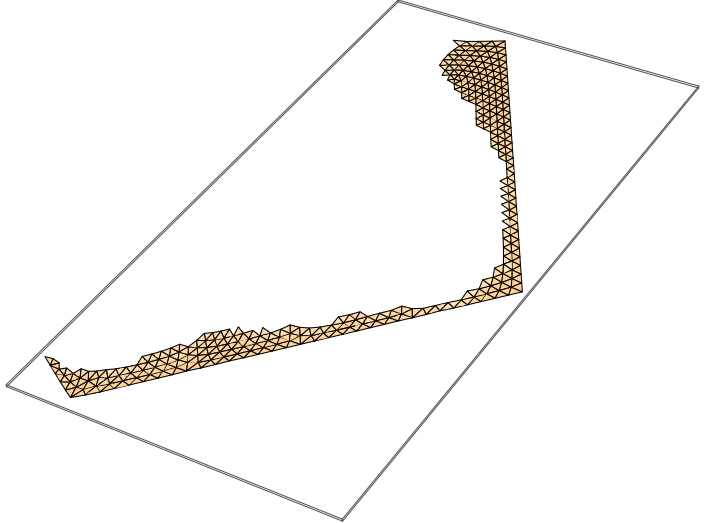
\includegraphics[width=12cm, height=6cm]{3DPolygonsImages/percolation-cluster-poly40.png}
\caption{The spanning cluster at the percolation threshold for the IWP of Figure~\ref{3Dpolygon40}. The water depth relative to the low point of the microtopography at the percolation threshold defines the depression depth.}
\label{perc-cluster-poly40}
\end{figure}

In summary, we hypothesize that the microtopographic effects on surface flow can be captured with a simple approximation with three parameters that can be computed from the microtopography:

\begin{itemize}
\item Subgrid relief $\delta_\text{max} = Z_{*,\text{max}} -   Z_{*,\text{min}}$, where  $Z_{*,\text{max}}$ and  $Z_{*,\text{min}}$ are the maximum and minimum elevation in the microtopography. 
\item Specific excluded volume $\delta_\text{ex}$, the soil volume above the microtopographic low point normalized by IWP area.
\item Depression depth $\delta$, the difference between the maximum and minimum elevation of the cells in the spanning cluster at the percolation threshold.
\end{itemize}
The subgrid releif and specific excluded volume come directly from the microtopography (univariate statistics). The depression depth requires a simple percolation algorithm to identify the spanning cluster at the percolation threshold.

\section{The Advanced Terrestrial Simulator (ATS)}\label{ATS}
\section{Results of Subgrid Model Simulations}\label{numerical-tests}

\section{Conclusions}\label{conclusion}

\section*{References}

\bibliography{reference}

\end{document}



